% !TeX encoding = UTF-8
% !TeX program = pdflatex
\documentclass[UTF8,a4paper,12pt]{ctexart}
\usepackage{times}
\usepackage[font=small,font=bf,labelsep=none]{caption} % 题注(caption)
%----------------------tab----------------------------------------------------
\usepackage{booktabs,diagbox,threeparttable}   % 三线表宏包,斜线表头,表格内加注释
\usepackage{array,multirow} % 制表环境,跨长的表格单元格
%-----------------------math-----------------------------------------------------
\usepackage{amsmath,amssymb,amsthm,mathrsfs,mathptmx, dutchcal} % math
\numberwithin{equation}{section}
\allowdisplaybreaks[4]       %多行公式中换页
%-------------------------------------------------------------------------
\usepackage{color, xcolor}  % 颜色支持
\usepackage{graphicx,subfigure}  %插图, PdfLaTeX 可以用png jpg pdf等,多图
\usepackage[subfigure]{tocloft}
\usepackage{tikz}
\usepackage{url}        % 超链接
% ----------------------间距------------------------------------------------
\usepackage{setspace}
\setlength{\baselineskip}{20pt} % 默认20pt
\newcommand*{\circled}[1]{\lower.7ex\hbox{\tikz\draw (0pt, 0pt)%
    circle (.5em) node {\makebox[1em][c]{\small #1}};}}
%----部分字体-----------------------------
\newcommand{\yihao}{\fontsize{26pt}{36pt}\selectfont}         % 一号, 1.4 倍行距
\newcommand{\erhao}{\fontsize{22pt}{28pt}\selectfont}         % 二号, 1.25倍行距
\newcommand{\xiaoer}{\fontsize{18pt}{18pt}\selectfont}        % 小二, 单倍行距
\newcommand{\sanhao}{\fontsize{16pt}{24pt}\selectfont}        % 三号, 1.5倍行距
\newcommand{\xiaosan}{\fontsize{15pt}{22pt}\selectfont}       % 小三, 1.5倍行距
\newcommand{\sihao}{\fontsize{14pt}{21pt}\selectfont}         % 四号, 1.5 倍行距
\newcommand{\banxiaosi}{\fontsize{13pt}{19.5pt}\selectfont}   % 半小四, 1.5倍行距
\newcommand{\xiaosi}{\fontsize{12pt}{18pt}\selectfont}        % 小四, 1.5倍行距
\newcommand{\dawuhao}{\fontsize{11pt}{11pt}\selectfont}       % 大五号, 单倍行距
\newcommand{\wuhao}{\fontsize{10.5pt}{15.75pt}\selectfont}    % 五号, 单倍行距
%--------------------------文献-------------------------------------------------
\usepackage[numbers]{gbt7714} %使用自有目录中的gbt7714.sty文件(宏包)
\usepackage{hyperref}  %目录
\hypersetup{colorlinks=true,linkcolor=black}
%----------------------------图表格式---------------------------------------------
\renewcommand {\thefigure} {\thesection{}-\arabic{figure}} %设定图片的编号。这样设置的实现效果为图1-1
\renewcommand {\thetable} {\thesection{}-\arabic{figure}}
\usepackage{caption}
\captionsetup{font={small},labelsep=quad}%文字5号,之间空一个汉字符位。
\captionsetup[table]{font={bf}} %表格表号与表题加粗
\usepackage{appendix}
%--------------------------------目录---------------------------------------------
\usepackage{tocloft}
\renewcommand{\cftsecleader}{\cftdotfill{\cftdotsep}} %为目录中section补上引导点
\usepackage{titletoc}
\titlecontents{section}[0pt]{\addvspace{6pt}\filright\bf}%
               {\contentspush{\thecontentslabel \quad}}%
               {}{\titlerule*[8pt]{.}\contentspage}
%--------------------页眉------------------------------------------------------------
\usepackage{fancyhdr} %页眉页脚
\pagestyle{fancy}
\fancyhf{}
\fancyfoot[R]{\thepage}
\makeatletter %双线页眉
\def\headrule{{\if@fancyplain\let\headrulewidth\plainheadrulewidth\fi%
\hrule\@height 1.5pt \@width\headwidth\vskip1.5pt%上面线为1pt粗
\hrule\@height 0.5pt\@width\headwidth  %下面0.5pt粗
\vskip-2\headrulewidth\vskip-1pt}      %两条线的距离1pt
  \vspace{6mm}}     %双线与下面正文之间的垂直间距
\makeatother
%----------------章节标题格式-------------------------------------------------------------
\CTEXsetup[format={\heiti \zihao{3} \bfseries \center}]{section}
\CTEXsetup[number={第\chinese{section}章}]{section}
\usepackage[explicit]{titlesec}
\titlespacing*{\section}{0pt}{24pt plus .24pt minus .24pt}{18pt plus .0ex}
%--------------------------带圈脚注-代码可以不管,能工作------------------------
\usepackage{pifont}
\usepackage[perpage,symbol*]{footmisc}
\DefineFNsymbols{circled}{{\ding{192}}{\ding{193}}{\ding{194}}
{\ding{195}}{\ding{196}}{\ding{197}}{\ding{198}}{\ding{199}}{\ding{200}}{\ding{201}}}
\setfnsymbol{circled}
%----------------------部分简写-------------------------------
\def\CnTitle{你的中文论文题目}
\def\EnTitle{你的英文论文题目}
\def\yemei{第十九届中国研究生电子设计竞赛~\\{\CnTitle}}
%%%%%%%%%%%%%%%%%%%%%%%%%%%%%%%%%%%%%%%%%%%%%%%%%%%%%%%%%%%%%%%%%%%%%%%%%%%%%%%%%%
%------------------------------------------------main------------------------------
\begin{document}

%-------------封面----------------------------------------------
\thispagestyle{empty}

\renewcommand{\headrulewidth}{0pt}


\begin{center}
\yihao{\textbf{第十九届中国研究生电子设计竞赛}} %1号黑体,居中
\yihao{\textbf{技术论文}}

\end{center}
%中文论文标题,1行或2行,宋体,加粗,二号,居中。论文题目不得超过36个汉字
~\\
\begin{center}
\xiaoer{\textbf{
\CnTitle
}}
~\\
~\\
\end{center}
\begin{center}
\xiaoer{\textbf{
\EnTitle
}}
\end{center}
%该页为中文扉页。无需页眉页脚,纸质论文应装订在右侧
~\\
~\\
~\\
~\\
\begin{center}
\heiti \zihao{-3}
\begin{tabular}{l}
\textbf{参赛单位:12356789}\\
~\\
\textbf{队伍名称:}\\
~\\
\textbf{指导老师:}\\
~\\
\textbf{参赛队员:}\\
~\\
\textbf{完成时间:}\\
\end{tabular}
\end{center}
~\\
%\begin{center}
%\songti \zihao{4} \textbf{20XX年XX月}
%\end{center}

%--------封面完毕-------------------------------------------

%------------------------------摘要-------------------------------------
\newpage
\pagenumbering{Roman}
\fancyhead[CH]{\songti \zihao{5} \yemei}
%\fancyhead[CH]{\songti \zihao{5}第十九届中国研究生电子设计竞赛~\\摘要}

\addcontentsline{toc}{section}{摘\quad要}
\section*{摘\quad要}
%摘要:二字间空一格,黑体16磅加粗居中,单倍行距,段前24磅,段后18磅。

\hspace{8mm}学位论文是研究生从事科研工作的成果的主要表现,集中表明了作者在研究工作中获得的新的发明、理论或见解,是研究生申请硕士或博士学位的重要依据,也是科研领域中的重要文献资料和社会的宝贵财富。\par
为了提高研究生学位论文的质量,做到学位论文在内容和格式上的规范化与统一化,特制作本模板。\\

\textbf{感谢上海交通大学的学位论文模板。}
~\\
\textbf{关键词}:学位论文,论文格式,规范化,模板\\
%关键字:宋体12磅,行距20磅,段前段后0磅,关键字之间用逗号隔开,关键词三个字加粗。

\newpage
%\fancyhead[CH]{\songti \zihao{5}第十九届中国研究生电子设计竞赛~\\ABSTRACT}
\addcontentsline{toc}{section}{ABSTRACT}
\section*{ABSTRACT}
%ABSTRCT:Arial 16磅加粗居中,单倍行距,段前24磅,段后18磅

\hspace{8mm}As a primary means of demonstrating research findings for postgraduate students, dissertation is a systematic and standardized record of the new inventions, theories or insights obtained by the author in the research work. It can not only function as an important reference when students pursue further studies, but also contribute to scientific research and social development.\par
This template is therefore made to improve the quality of postgraduates’ dissertation and to further standardize it both in content and in format.\\
%英文摘要内容:Times New Roman 12磅,行距20磅段前段后0磅
~\\
\textbf{Key words}: dissertation, dissertation format, standardization, template
%Keywords:Times New Roman 12磅,行距20磅, “key words” 两词加粗

%----------------------------------目录-----------------------------------------------------
\newpage
%\fancyhead[CH]{\songti \zihao{5}第十九届中国研究生电子设计竞赛~\\{中文论文题目}}
\fancypagestyle{plain}{
  \pagestyle{fancy}
}
\renewcommand\contentsname{\textbf{目\quad 录}}
\begin{center}
{\tableofcontents %增加章节目录...
}
\end{center}

%---------------------------------------------------------------------
%------------------------正文--------------------------------------1
\newpage
\pagenumbering{arabic} %阿拉伯,右下角
\pagestyle{fancy}
\fancyhf{}
\fancyfoot[R]{\thepage}
\fancyhead[CH]{\songti \zihao{5} \yemei}
%--------------------第 1 章------------------------------------------------
\section{绪论}
\subsection{引言}
学位论文……
\subsection{本文主要研究内容}
本文……
\subsection{本文研究意义}
本文……
\subsection{引用文献的标注}
样式包%
\footnote{\url{https://www.ctan.org/pkg/biblatex-gb7714-2015}}%
控制参考文献的输出样式。
研电赛\cite{liu2021}是什么。
可能需要一点人工智能的驱动\cite{ouyang2021t,tang2020q}。


\subsection{本章小结}
本文……

\newpage
%---------------------第 2 章------------------------------------------------
\section{正文文字格式}
\subsection{论文正文}
论文正文是主体,一般由标题、文字叙述、图、表格和公式等部分构成。一般可包括理论分析、计算方法、实验装置和测试方法,经过整理加工的实验结果分析和讨论,与理论计算结果的比较以及本研究方法与已有研究方法的比较等,因学科性质不同可有所变化。\par
论文内容一般应由十个主要部分组成,依次为:⒈封面,⒉中文摘要,⒊英文摘要,⒋目录,⒌符号说明,⒍论文正文,⒎参考文献,⒏附录,⒐致谢,⒑攻读学位期间发表的学术论文目录。\par
以上各部分独立为一部分,每部分应从新的一页开始,且纸质论文应装订在论文的右侧。\par
\subsection{字数要求}
\subsubsection{硕士论文字数要求}
各学科和学部自定
\subsubsection{博士论文字数要求}
各学科和学部自定
\subsection{本章小结}
本章介绍了……

\newpage
%--------------------第3章------------------------------------------------
\section{图表、公式格式}
\subsection{图表格式}

\begin{figure}[htb]
\center{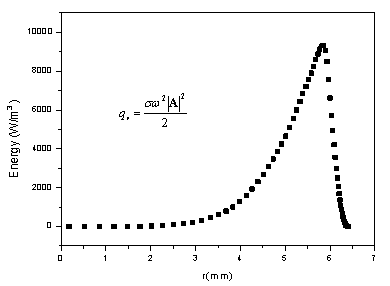
\includegraphics[width=0.95\textwidth]  {fig2.png}}
\caption{内热源沿径向的分布}
\end{figure}

\begin{table}[!htbp]
\centering
\caption{高频感应加热的基本参数}
\begin{tabular}{|c| c|c|c|}
\hline
感应频率 &感应发生器功率 & 工件移动速度  &感应圈与零件间隙\\
(KHz)&($\% \times$80Kw) &(mm/min)  &(mm)\\
\hline
250 &88 &5900 &1.65\\
\hline
250 &88 &5900 &1.65\\
\hline
250 &88 &5900 &1.65\\
\hline
250 &88 &5900 &1.65\\
\hline
250 &88 &5900 &1.65\\
\hline
250 &88 &5900 &1.65\\
\hline
250 &88 &5900 &1.65\\
\hline
250 &88 &5900 &1.65\\
\hline
\end{tabular}
\end{table}

\begin{table}
\centering
\captionsetup{singlelinecheck=off}
\caption*{续表} %取消编号
\begin{tabular}{|c| c|c|c|}
\hline
感应频率 &感应发生器功率 & 工件移动速度  &感应圈与零件间隙\\
(KHz)&($\% \times$80Kw) &(mm/min)  &(mm)\\
\hline
250 &88 &5900 &1.65\\
\hline
250 &88 &5900 &1.65\\
\hline
\end{tabular}
\end{table}
%表格太大需要转页时,需要在续表上方注明“续表”,表头也应重复排出。


\subsection{公式格式}

\vspace{-10mm}
\begin{eqnarray}
\frac{1}{\mu} \nabla^2A - j \omega \sigma A -\nabla(\frac{1}{\mu}) \times(\nabla \times A)+J_0=0
\end{eqnarray}

\subsection{本章小结}
本章介绍了……

\newpage
%--------------------第*章------------------------------------------------
\section{全文总结}

\subsection{主要结论}
本文主要……

\subsection{研究展望}
更深入的研究……

%----------------------------------参考文献-----------------------------------
\newpage


\addcontentsline{toc}{section}{参\quad考\quad文\quad献}
\renewcommand\refname{参\quad考\quad文\quad献}
\begin{spacing}{1.2} % 行距
	\zihao{5} \songti
    %\bibliographystyle{gbt7714-unsrt}
	\bibliography{yds}
	\vspace{11bp}
\end{spacing}


\newpage

\end{document} 